\documentclass[conference]{IEEEtran}
\IEEEoverridecommandlockouts

\usepackage[english]{babel}
\addto\captionsspanish{\renewcommand{\tablename}{Tabla}}
\usepackage[utf8]{inputenc}
\usepackage[T1]{fontenc}
\usepackage{cite}
\usepackage{amsmath,amssymb,amsfonts}
\usepackage{graphicx}
\usepackage{xcolor}
\usepackage{textcomp}
\usepackage{tikz}
\usepackage{array}
\usepackage{booktabs}
\usepackage{url}
\usetikzlibrary{positioning, arrows.meta, shapes, fit}

\newcommand{\pend}[1]{\textcolor{red}{[#1]}}

\begin{document}

\title{Optimization of Depth-First Search Algorithms\\
on 2D Matrices using a RISC-V Processor\\
with Hardware Acceleration}

\author{
\IEEEauthorblockN{Gabriel Abarca Aguilar, Jes\'us Alberto Castro Murillo,
Jos\'e Fabio Jaramillo Cordero,\\ Mois\'es Leiva Solano and Noel Antonio P\'erez C\'aceres}
\IEEEauthorblockA{\textit{School of Electronic Engineering}\\
\textit{Instituto Tecnol\'ogico de Costa Rica}\\
Costa Rica}
}

\maketitle

\begin{abstract}
\textit{Depth-First Search} (DFS) is a fundamental traversal primitive over 2D
matrices, underlying problems such as connected-component labeling,
\textit{flood fill}, and pattern search on grids. Its sequential nature and
irregular memory accesses limit performance on general-purpose processors. This
work proposes to optimize DFS algorithms over 2D matrices using a RISC-V
processor with hardware acceleration, modeled at a high level in SystemC to
enable early architectural exploration. Based on the analysis of several DFS
problems, the dominant computation pattern is identified as a candidate for
specialization. The resulting accelerator is modeled in SystemC/TLM~2.0 and
synthesized to RTL for an AMD Kria KV260 through Vitis HLS. Across five
representative DFS problems and their variants (21 cases), the accelerator
matches the RISC-V software baseline exactly, confirming its functional
correctness, while the SystemC-level cost model predicts a
1.33$\times$--4.00$\times$ speedup. On the real board, however, the
accelerator does not yet beat the software baseline: measured speedup ranges
from 0.01$\times$ to 0.27$\times$, improving with problem size but never
crossing 1$\times$ at the largest supported grid. An independent,
cycle-accurate co-simulation confirms this gap is real and traces it to two
causes external to the DFS logic: a $\sim$12{,}000~ns fixed overhead per
invocation over AXI/DMA, and a memory access pattern that runs two
synthesized loops 16$\times$ slower than intended. The accelerator itself
uses under 13\% of the FPGA fabric and closes timing at 204~MHz, leaving room
to close this gap in future work.
\end{abstract}

\begin{IEEEkeywords}
Depth-First Search, RISC-V, hardware acceleration, 2D matrices, SystemC,
architectural exploration.
\end{IEEEkeywords}

\section{Introduction}

\textit{Depth-First Search} (DFS) is a fundamental traversal algorithm in
computer science, and is the core of multiple problems defined over 2D matrices
\cite{datacamp_dfs}. By mapping each value of the matrix as a connected node,
DFS allows us to discover connectivity, regions, and paths within it. We can
find this kind of approach in robotics, video games, image processing,
discrete-space planning, and connected-component labeling.

DFS efficiency depends on the problem. In a simple graph traversal, where each
node is visited once, the cost is $O(m \cdot n)$ for an $m \times n$ matrix
\cite{datacamp_dfs}. But other problems launch a separate DFS from every single node. Here the cost is no longer linear: with
$m \cdot n$ origins, a branching factor $b$, and a maximum path length $L$, the
work grows as $O(m \cdot n \cdot b^{L})$, exponentially with path length. This
makes DFS a bottleneck in these applications and justifies exploring parallelism
options across the independent searches.

These costs intensify in general-purpose hardware. Matrix and graph traversal
has irregular memory accesses and low arithmetic intensity, which reduces
performance on CPUs, as their cache hierarchies fail to exploit locality
\cite{giorgi2023, dann2021}. Also, on platforms with limited memory the stack
and the visited set may not fit in internal memory, so data is repeatedly
transferred and transfer time dominates compute time \cite{giorgi2023}. The
sequential nature of DFS also limits parallelism. Since the traversal state is
shared, multiple threads over a single memory increase contention overhead
rather than improving performance \cite{giorgi2023}. For this reason,
specialized architectures have been adopted that tailor the \textit{datapath}
and memory to the traversal's access pattern \cite{dann2021}.

In this paper we work on making DFS faster over 2D matrices, using a RISC-V
processor with hardware acceleration that we model in SystemC. The main idea is to identify, in the code of multiple DFS problems, the leading
algorithmic pattern and adapt the processor to execute it in an efficient way,
using the core as an orchestrator. Our contributions are threefold. (i) An analysis of the algorithmic pattern
shared across DFS problems, identifying promising candidates for acceleration.
(ii) An architecture and its SystemC model for design-space exploration before
RTL. (iii) An experimental methodology to compare the solution against a
baseline RISC-V execution, reporting \textit{throughput}, latency, and resource
metrics.

%=========================================================================

\section{Background and Related Work}

Current research has addressed the acceleration of depth-first search (DFS) and 
graph traversal from three complementary approaches: parallelization of the traversal, 
optimization of memory access, and hardware specialization.

\subsection{Traversal Parallelization}

A common approach is to find independent tasks that can be executed in multiple flows. Futuhi and Sturtevant 
propose a CPU-GPU framework for cost-bounded DFS that separates the search and 
heuristic evaluation phases, groups evaluations into batches, and distributes subtree 
among asynchronous workers. Running the heuristic checks in GPU batches makes cost-bounded DFS tens of times
faster than doing them one at a time, on problems like the Rubik's Cube and the
sliding-tile puzzle \cite{futuhi2025}. 

Their approach suggests that the phases of a DFS can be separated and distributed, 
an idea we reuse when offloading the computation to hardware. 
Naumov \textit{et al.} approach the problem from the perspective of 
graph structure. They present an efficient parallel algorithm that traverses a directed 
acyclic graph in a manner similar to BFS—up to three times—to obtain the preorder, postorder, 
and parent relationships for each node. Their CUDA implementation achieves up to a $6\times$ 
speedup compared to sequential DFS on a CPU\cite{naumov2017}. 

This work provides us with a concrete technique for extracting parallelism from a 
traversal that is theoretically considered sequential. Yuan \textit{et al.} extend 
this idea to subgraph matching. They organize the search into a non-blocking task 
queue distributed across GPU warps, introduce a timeout mechanism that reassigns tasks 
to maintain load balance, and employ dynamic memory allocation for stack spaces~\cite{yuan2024}. 
From this, we adopt the approach to managing load imbalance among branches of unequal 
depth—a central problem in DFS. Taken together, these works confirm that DFS exposes 
task-level parallelism. However, they all rely on CPU+GPU platforms and state spaces 
other than the dense 2D matrices addressed by this proposal.


\subsection{Optimizing Memory Access and Locality}

Dann \textit{et al.} have conducted a detailed study on how various FPGA-based 
graph accelerators access memory. Speed depends on two things: how much the accelerator is being used and how the data is handled in memory. Based 
on this, they point out that techniques such as partitioning data, processing 
independent regions, and improving spatial and temporal locality can significantly 
reduce access time \cite{dann2021}. Their contribution is a catalog of memory factors 
that a traversal accelerator must take into account.

Mukkara \textit{et al.} have developed a mechanism based on this analysis: they have introduced 
\textbf{BDFS} (Bounded Depth-First Scheduling), a locality-aware scheduling strategy that keeps each core
working on one connected region of the graph at a time. They also built \textbf{HATS},
a hardware-accelerated traversal scheduler that runs this strategy and improves performance by up to $3.1\times$ over a locality-oblivious baseline \cite{mukkara2018}.


This work follows a philosophy similar to ours: instead of reordering vertices 
in a general graph, it specializes the datapath of a RISC-V core to execute the 
dominant traversal pattern on 2D matrices. SeqDFS pursues the same goal through 
software, reordering the visit sequence of vertices to improve cache efficiency 
and reduce the cost of traversing sparse graphs~\cite{Lyu2021SeqDFS}. Both agree 
that the order of visitation is key to optimizing the traversal.

Giorgi \textit{et al.} have addressed the limitation of devices' internal memory: since this 
forces repeated data transfers, causing transfer time to exceed computation time, 
they propose dividing the graph and using a distributed multi-FPGA architecture that 
outperforms equivalent implementations on CPUs and GPUs~\cite{giorgi2023}.

\subsection{Specialization in reconfigurable hardware}

A third approach maps its control logic to dedicated \textit{hardware}. Mukherji \textit{et al.} 
implement a DFS on an FPGA as part of a Huffman encoding accelerator, demonstrating in this way that the path can be mapped to reconfigurable hardware
\cite{mukherji2025};  Mahammad et al. reinforce this approach with a dual dynamic tree selection Huffman encoder 
on an FPGA that reduces latency and resource usage compared to previous work, achieving high throughput in image processing applications \cite{article}. 
Both validate the relevance of specialized hardware for embedded systems where speed and resource usage are critical. 
In the domain of \textit{backtracking}, Davis \textit{et al.} offload the constraint propagation 
loop from a SAT solver to an FPGA inference engine that stores the instance in Block RAM and 
partitions the problem among several engines in parallel. The accelerator infers implications
in 6 to 17 clock cycles and is 5 to 16 times faster than the equivalent solution in Microsoft SAT software \cite{microsoftsat}. 
Their contribution proves that the forward-backtracking loop—the heart of backtracking—can be executed on a dedicated
\textit{datapath} with substantial gains. However, these designs address domains whose data structures and pruning logic differ from traversal on 2D arrays.


\subsection{Strengths and Weaknesses of State-of-the-Art (SOTA) Solutions}

Table~\ref{tab:sota_fortalezas} summarizes, by line of attack, the
strengths and weaknesses identified in Section~II, along with the
conditions that make each approach viable (or not) for the dense 2D
matrix DFS problem tackled in this work. We also bring in three
additional lines not covered in the original review: graph-oriented
RISC-V ISA extensions (Yenimol~et~al.~\cite{yenimol2022} and
GPGCN~\cite{tang2022gpgcn}), FPGA-based connected component labeling
(CCL/CCA) accelerators (Union-Retire~\cite{bailey2022unionretire},
CCL~4K~\cite{kowalczyk2021ccl4k}, and
Run-Length~CCA~\cite{appiah2008runlength}), and sparse graph traversal
accelerators on FPGA with high-bandwidth memory
(ScalaBFS2~\cite{li2024scalabfs2}). These are included because they share
the same underlying neighborhood exploration pattern over graph or matrix
structures as our DFS traversal.

\begin{table*}[t]
\centering
\footnotesize
\caption{Strengths, weaknesses, and viability of SOTA solutions, by line of attack.}
\label{tab:sota_fortalezas}
\renewcommand{\arraystretch}{1.0}
\begin{tabular}{@{}p{2.6cm}p{0.9cm}p{4.6cm}p{4.6cm}p{4.0cm}@{}}
\toprule
\textbf{Line} & \textbf{Refs.} & \textbf{Strengths} & \textbf{Weaknesses / not viable when\ldots} & \textbf{Viable when\ldots} \\
\midrule
 
Traversal parallelization (CPU+GPU)
& \cite{futuhi2025}, \cite{naumov2017}, \cite{yuan2024}
& Order-of-magnitude gains in bounded DFS; up to 6$\times$ in CUDA. Mitigates load imbalance between branches.
& Needs a CPU+GPU platform, ruling out embedded cores; inefficient on regular 2D matrices.
& A GPU is available and the domain needs a general graph or a costly-metric space. \\

Memory optimization and locality
& \cite{giorgi2023}, \cite{dann2021}
& Identifies key memory bottlenecks; Giorgi's multi-FPGA setup beats CPU/GPUs past one chip's capacity.
& Dann has no hardware proposal; Giorgi loses efficiency past capacity. Both target sparse, PageRank-like methods, not dense DFS.
& The graph exceeds one FPGA's capacity and the algorithm is iterative, PageRank-like. \\

Specialization in reconfigurable hardware (Huffman/SAT)
& \cite{mukherji2025}, \cite{article}, \cite{microsoftsat}
& 5--16$\times$ over software with minimal LUTs, in SAT and Huffman.
& DFS engine fused with domain logic; cannot reuse it as a generic search engine.
& The problem is fixed to compression or SAT, with rules known upfront. \\

RISC-V ISA extension for graphs
& \cite{yenimol2022}, \cite{tang2022gpgcn}
& Custom instructions without losing speed; GPGCN hits 1001$\times$ over CPUs, 267$\times$ over vector extensions (Cora).
& Yenimol has no chip or empirical data; GPGCN is CSR-only, unlike a DFS stack.
& Proof of concept that ISA changes help, but not a direct DFS alternative. \\

Connected component labeling (CCL/CCA) on FPGA
& \cite{bailey2022unionretire}, \cite{kowalczyk2021ccl4k}, \cite{appiah2008runlength}
& Minimal-hardware flood fill: Union-Retire cuts memory 36\,\%, Kowalczyk hits 4K/60~fps, Run-Length beats software.
& Single raster pass, no stack or backtracking; Union-Retire needs more logic, Kowalczyk struggles with concurrent merges.
& The matrix is strictly binary and solvable in one linear sweep. \\

Sparse graph accelerators on FPGA with HBM
& \cite{li2024scalabfs2}
& HBM crossbar pushes BFS to 56.92~GTEPS, 3$\times$ its predecessor, matching high-end GPUs at half the bandwidth.
& Needs costly HBM boards, unlike the KV260; tailored for sparse BFS; crossbar scales quadratically on dense matrices.
& HBM budget available and the bottleneck is random access over massive sparse graphs. \\
\bottomrule
\end{tabular}
\end{table*}

\subsection{Observed Challenges}
From the analysis in Section II and the summary in Table I, we can pull out the main problems that pushed us to do this work. 
The first challenge focuses on the fact that DFS parallelism is limited by contention on the shared traversal state.
Second, traversal of 2D matrices exhibits an irregular memory access pattern, which reduces cache utilization and increases latency in the architectures. 
Third, state-of-the-art solutions focus primarily on sparse graphs, GPU acceleration, or specialized domains such as SAT or subgraph matching. 
This limits their direct applicability to the problem of DFS on dense 2D matrices in a RISC-V-based embedded environment. 
Taken together, these limitations highlight the absence of a specialized architecture that decouples DFS control from neighbor exploration computation, which defines the architectural gap that this work addresses in the following section.

%=========================================================================

\section{Proposed Solution}

\subsection{DFS Accelerator Operation Flow}

The proposed architecture implements a hardware accelerator for the execution of the Depth First Search (DFS)
algorithm on 2D arrays. The system shifts the computational load from the processor to the FPGA unit,
composed of 3 stages: control, exploration, and storage modules.

The complete implementation is publicly available in the project
repository.\footnote{\url{https://github.com/Team-Diseno-de-Alto-Nivel/mp6160-riscv-dfs-accelerator}}

The search state is stored in the following stages:

\begin{figure}[h]
    \centering
    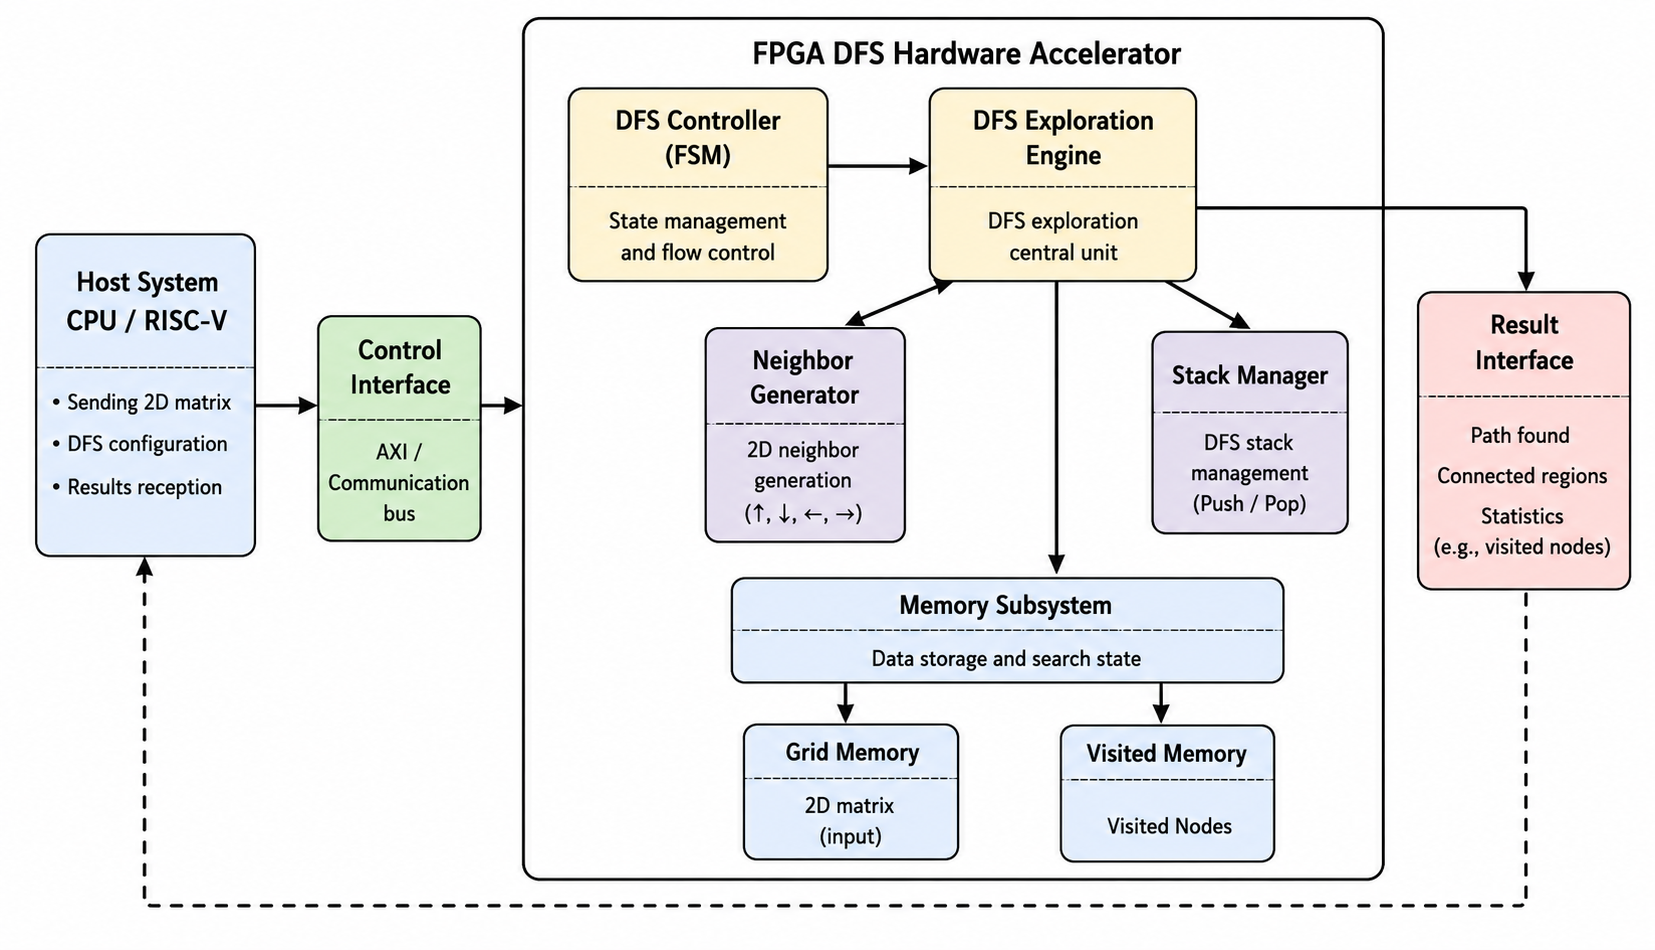
\includegraphics[scale=0.15]{images/diagrama_segundo_nivel2.png}
    \caption{Proposed architecture of the DFS hardware accelerator for 2D matrix scanning.
            The system separates the execution of the DFS algorithm from the main processor using a
            specialized FPGA engine composed of control, scanning, and memory modules.}
    \label{fig:diagrama_segundo_nivel}
\end{figure}

\subsubsection{Configuration and data loading}

Initially, the host system, based on a CPU/RISC-V processor, sends the information 
necessary to initiate the search. This information includes the input 2D grid, the 
initial traversal position, and the algorithm's configuration parameters. The grid 
is stored in the \textit{grid memory}, while the \textit{visited memory} is initialized to prevent 
repeated traversals.

\subsubsection{DFS Controller}

The DFS Controller controls the operation sequence of the accelerator by a finite state machine (FSM). This controller handles the phases of reading nodes, exploring neighbors, updating the memory state and ending the traversal. This maintains the flow of execution of the DFS algorithm without intervention from the processor.

\subsubsection{Neighbor Generation}

The Neighbor Generator module is responsible for obtaining the positions 
adjacent to the current node within the 2D matrix. For a cell at position $(x,y)$, the hardware produces its four neighbors: $(x-1,y)$, $(x+1,y)$, $(x,y-1)$, and $(x,y+1)$. Doing this in hardware avoids recomputing neighbors over and over in software.

\subsubsection{Stack Manager}

Due to the iterative nature of the DFS algorithm, it is necessary to maintain a
record of the unexplored nodes. The Stack Manager module implements this function using
push/pop operations, allowing the traversal order to be preserved and the internal state of the
search to be efficiently managed.

\subsubsection{Memory subsystem}

During the scan, the accelerator accesses internal memories
to query the grid information and update visited nodes.
The separation between Grid Memory and Visited Memory allows the input information 
and the dynamic state of the algorithm to remain independent, preventing redundant scans.

\subsubsection{Result Interface}

Finally, when there are no more pending nodes in the stack, the controller
terminates execution and the \textit{Result Interface} module delivers the generated
information to the host system. Depending on the application, the result
can represent a path found, connected region, or the number of nodes explored.

\subsection{Development Flow}

The proposed DFS accelerator was developed following a hardware design methodology in which functional validation was prioritized. The project starts from the description of the high-level software instead of implementing the architecture directly in RTL, and is then refined into a hardware-oriented model. This development strategy reduces debugging effort and allows architectural exploration at the early stage.

This development follows a refinement methodology, in which the accelerator moves forward from a software reference into a FPGA-based hardware system. Figure~\ref{fig:development_flow} illustrates the stages.


\begin{figure}[h]
\centering

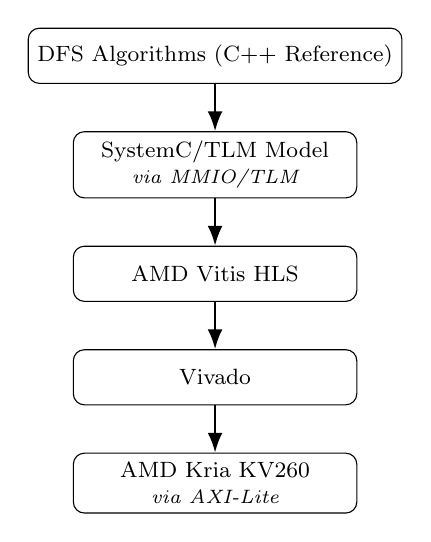
\begin{tikzpicture}[
node distance=0.6cm,
block/.style={
rectangle,
draw,
rounded corners,
minimum width=3.6cm,
minimum height=0.7cm,
align=center,
font=\footnotesize
},
arrow/.style={
-{Latex[length=2.5mm]},
thick
}
]

\node[block] (dfs) {DFS Algorithms (C++ Reference)};
\node[block, below=of dfs] (systemc) {SystemC/TLM Model \\ {\scriptsize\itshape via MMIO/TLM}};
\node[block, below=of systemc] (hls) {AMD Vitis HLS};
\node[block, below=of hls] (vivado) {Vivado};
\node[block, below=of vivado] (kv260) {AMD Kria KV260 \\ {\scriptsize\itshape via AXI-Lite}};

\draw[arrow] (dfs) -- (systemc);
\draw[arrow] (systemc) -- (hls);
\draw[arrow] (hls) -- (vivado);
\draw[arrow] (vivado) -- (kv260);

\end{tikzpicture}

\caption{Development flow: from a C++ reference through SystemC/TLM, HLS, and Vivado onto the KV260. The host drives the design via MMIO/TLM in simulation and via AXI-Lite once on hardware.}
\label{fig:development_flow}

\end{figure}

The modeling language used during the early stages was SystemC, the main objective was to verify the behavior of the DFS architecture before moving into an RTL implementation. The use of SystemC/TLM enabled the communication model between the hardware modules and the verification of the accelerator while preserving a higher level of abstraction.

SystemC also enables early design evaluation by architectural exploration and latency analysis before synthesis. This shortens the time of development and enables comparison of different approaches and design improvements.

The accelerator was designed in a modular architecture, not as a complex block, to make it future hardware optimization, maintainability and scalability friendly. Each module has a specific function and communicates with the other modules of the system via interfaces. This organization offers a structure similar to a real hardware accelerator.

\subsection{Accelerator Architecture}

The accelerator architecture is composed of independent hardware modules controlled by a centralized DFS controller, as shown in Figure~\ref{fig:diagrama_segundo_nivel}.

The communication between software and hardware accelerator is modeled through a memory-mapped register interface using Transaction-Level Modeling (TLM). From the software perspective, the accelerator behaves as a memory-mapped peripheral, while internally the SystemC model captures the interactions among the hardware modules.
The communication scheme follows a structure similar to an AXI-Lite peripheral; the transition from the SystemC model to the FPGA implementation requires only minor architectural changes, which reduces the hardware integration effort and lets the validated model be reused during the synthesis stages.


\subsection{Hardware Generation Strategy}

Instead of using the traditional RTL design, the AMD Vitis High-Level Synthesis (HLS) tool was selected for hardware generation. This decision helps reduce development complexity and allows the hardware implementation to start from a higher-level behavioral description. After the SystemC model has been functionally validated and its timing characteristics have been analyzed, the design can be further synthesized into RTL using Vitis HLS. This enables a smoother transition from architectural modeling to hardware implementation while preserving the validated functionality.
Using HLS also allows the application of hardware-specific optimizations, such as loop pipelining, interface generation, and resource utilization improvements without compromising code  long-term maintainability and readability.

\subsection{Target Platform Selection}
The AMD Kria KV260 was selected as the target platform because it provides a suitable environment for hardware/software co-design and FPGA-based deployment.
The combination of programmable logic, an embedded processing system, AXI-based communication infrastructure, and native support for the AMD Vitis toolchain makes the KV260 a suitable platform for integrating and evaluating custom hardware accelerators \cite{amd_kv260_user_guide, amd_vitis_hls_user_guide}.
Additionally, the communication architecture adopted throughout this project is compatible with the AXI-based infrastructure available on the KV260 platform \cite{arm_axi_protocol}. This compatibility simplifies the integration process and enables a direct transition from the SystemC model to the final FPGA implementation.

\subsection{Hardware/Software Integration}

Altogether, these design choices define a complex development methodology that ranges from the validation of algorithms, to architectural modeling, hardware synthesis and FPGA deployment.

By validating the accelerator functionality and performance before generating the RTL implementation, the proposed workflow increases confidence in the correctness of the design while reducing development complexity and enabling future improvements or extensions to the architecture.

\section{Results and Analysis}

\subsection{Experiment Plan}

To benchmark the proposed solution against a RISC-V baseline, five DFS problems
over 2D matrices were selected from LeetCode \cite{leetcode}. They cover the
algorithmic patterns identified in Section~II. Each is executed with varied
inputs to force its worst case, measuring the cost in simulated cycles for
different matrix sizes.

\begin{itemize}
\item \textbf{Number of Islands}: counts regions of connected cells in a binary
matrix using a flood fill that marks each visited cell and expands to its
neighbors. Connectivity (4 and 8 neighbors) and island density are varied to
measure the cost of the pattern in the best and worst cases.
\item \textbf{Unique Paths III}: counts the paths that visit every walkable cell
exactly once, using backtracking that marks and unmarks visited cells. Obstacle
density and matrix size are varied to measure the cost
up to the point where it becomes impractical.
\item \textbf{Word Search II}: determines which words from a list can be formed
by traversing adjacent cells without repeating them, using backtracking guided
by a shared trie that skips branches without a valid prefix. Dictionary size is
varied and pruning is removed to measure the cost with and without that
algorithmic optimization.
\item \textbf{Longest Increasing Path}: finds the length of the longest path
with strictly increasing values, using multi-source DFS with \textit{top-down}
memoization to avoid recomputing subpaths. It is run with and without
memoization to measure the cost of the exponential search against its bounded
version.
\item \textbf{Pacific Atlantic Water Flow}: finds the cells from which water can
flow to both oceans on opposite edges of the matrix, using multi-source DFS
launched from the edges with two visited sets that intersect at the end. The
matrix shape, square or narrow, is varied to measure the cost of that
edge-anchored search.
\end{itemize}

The proposed accelerator can be turned on or off at runtime, so each case runs
twice on the same model, once with the accelerator on and once with just the
RISC-V core, and both runs record:

\begin{itemize}
\item Simulated latency (\texttt{sc\_time})
\item Instruction count
\item \textit{Throughput} (cells processed per second)
\item Visited cells and expanded nodes
\item Peak stack depth
\end{itemize}

Hardware-level metrics from synthesizing and implementing the
accelerator on the FPGA were collected, including:

\begin{itemize}
\item Resource usage (LUT, FF, BRAM, and DSP)
\item Maximum operating frequency (\textit{Fmax}) and \textit{timing} closure
\item Sustained \textit{throughput} in operations per second (OP/s)
\end{itemize}

A metric-by-metric comparison of the two runs quantifies the gain provided by
the accelerator. The model is implemented in SystemC 2.3.4 with TLM~2.0, and the
software is compiled with \texttt{riscv64-unknown-elf-gcc/g++}. The hardware generation strategy and target platform are detailed in
Section~III.

\subsection{Preliminary Results}

The experiment plan above has been executed end to end: the RISC-V software
baseline and the real, synthesizable SystemC/TLM~2.0 accelerator model (not a
behavioral stand-in) were co-simulated over the same TLM~2.0 register
interface used by the hardware, for all five problems and their variants,
with the accelerator off and on. Every one of the 21 resulting cases matches
the software baseline exactly, confirming that the accelerator logic is
correct ahead of physical implementation. Table~\ref{tab:prelim_results}
summarizes the simulated-latency speedup observed per problem; the
per-case data (instruction count, throughput, visited cells, and peak
stack depth) is in the project repository.

\begin{table}[h]
\centering
\caption{Preliminary speedup (accelerator on vs.\ off), simulated latency.}
\label{tab:prelim_results}
\renewcommand{\arraystretch}{1.15}
\begin{tabular}{@{}p{3.55cm}cc@{}}
\toprule
\textbf{Problem (variant)} & \textbf{Cases} & \textbf{Speedup range} \\
\midrule
Number of Islands & 6 & 1.39$\times$--1.97$\times$ \\
Unique Paths III & 3 & 1.47$\times$--1.50$\times$ \\
Word Search II & 2 & 1.47$\times$--1.60$\times$ \\
Word Search II (no pruning) & 2 & 1.55$\times$--1.67$\times$ \\
Longest Increasing Path & 3 & 4.00$\times$ (constant) \\
Longest Increasing Path (no memo) & 3 & 4.00$\times$ (constant) \\
Pacific Atlantic & 2 & 1.33$\times$--1.50$\times$ \\
\bottomrule
\end{tabular}
\end{table}

Two patterns stand out. First, \textit{Number of Islands} gains more from the
accelerator on denser, more fragmented grids (checkerboard, 1.60--1.97$\times$)
than on a single connected region (1.39--1.47$\times$): the more islands the
multi-source scan has to restart from, the more of the traversal's
visited/neighbor bookkeeping the controller takes over from the software.
Second, \textit{Longest Increasing Path} shows an exact, constant
4$\times$ speedup regardless of memoization. That problem is driven entirely
through the fine-grained primitive interface (\textit{is\_visited},
\textit{mark\_visited}, \textit{neighbours}), so the ratio reflects the fixed
per-primitive cost difference between the software and accelerator paths in
the simulation's cost model, not an algorithm-dependent effect.

The theoretical model failed to accelerate processing on the AMD Kria
KV260 board, resulting in a tenfold speed reduction due to a 90--100\%
underestimation of latency by the cost model (Table~\ref{tab:cost_model_correlation}).
At this scale, the overhead comes from invoking the accelerator itself,
rather than the DFS computation.

The cost model only considers the cost of the operations involved in the
DFS traversal itself, not the fixed cost of calling the accelerator over
AXI, which is register writes, the interrupt round trip and the transfer
of the result via DMA, all of which adds up to a minimum of
$\sim$12{,}000 ns per invocation, independent of the problem size. This
is not a measurement error: the cost model itself was optimistic. The
independent Vitis HLS cycle-accurate co-simulation estimate is
128--10{,}811 cycles (640--54{,}055 ns at 200 MHz), in the same order of
magnitude as the hardware measurement. Closing this gap would require an additive fixed-overhead term in the
cost model, not just retuning \texttt{cycles\_per\_op}/\texttt{clock\_period\_ns}.

\begin{table}[h]
\centering
\footnotesize
\caption{Simulated (modelled) vs.\ on-board (measured) speedup.}
\label{tab:cost_model_correlation}
\renewcommand{\arraystretch}{1.15}
\begin{tabular}{@{}p{3.1cm}ccc@{}}
\toprule
\textbf{Problem (variant)} & \textbf{Model.} & \textbf{Meas.} & \textbf{Error} \\
\midrule
Number of Islands & 1.65$\times$ & 0.07$\times$ & +96.0\% \\
Unique Paths III & 1.48$\times$ & 0.09$\times$ & +90.3\% \\
Word Search II & 1.54$\times$ & 0.04$\times$ & +97.4\% \\
Word Search II (no pruning) & 1.61$\times$ & 0.04$\times$ & +97.7\% \\
Pacific Atlantic & 1.41$\times$ & 0.06$\times$ & +90.9\% \\
Longest Increasing Path & 4.00$\times$ & 0.01$\times$ & +99.6\% \\
Longest Increasing Path (no memo) & 4.00$\times$ & 0.02$\times$ & +99.2\% \\
\midrule
\textbf{Aggregate} & \textbf{1.56$\times$} & \textbf{0.10$\times$} & \textbf{+96.0\%} \\
\bottomrule
\end{tabular}
\end{table}

To determine if this gap shrinks with problem size, the same test ran on
64$\times$64 grids (4,096 cells), the largest size the kernel supports,
instead of the small legacy cases. Measured speedup improves from
0.10$\times$ to 0.27$\times$, and the latency error drops from
$\sim$97\% to 21--83\%, depending on the problem. The fixed overhead
does shrink as the problem grows, but even at the largest size the
hardware supports, it still does not beat the software baseline.

Splitting an invocation into its three steps -- start, wait, and read
the result back -- shows the wait step takes 97.1\% of the time; start
and read-back are 1.7\% and 1.1\%. Batching the read-back step barely
changes latency (1.4\%), so that is not the cause. The wait step is not
wasted time, though: part of it is real computation. Using the case
with almost no work as a baseline ($\sim$12,240 ns), the leftover
computation time for the 4,096-cell case is $\sim$273,000 ns -- about
double what the cost model predicts. So there are two separate gaps: a
fixed cost per call and a slower-than-expected computation itself.

Both are specific hardware causes, not open-ended questions. The kernel
cannot start a new run until the current one is finished, so the issue
cannot be fixed in software alone. The synthesis report alone already
shows two loops running 16 times slower than intended due to a memory
access pattern, a clear target for future work. Neither is fixed in
this iteration.

Table~\ref{tab:resource_utilization} reports the post-implementation
resource usage on the KV260 (Vivado, 200~MHz operating frequency). The
accelerator uses a modest share of the fabric -- under 13\% of any
resource class -- leaving headroom for the memory-access fix identified
above. Timing closes with positive slack at 204~MHz (WNS +0.084~ns),
which is the demonstrated maximum rather than the 200~MHz operating
point used on-board, where the sustained throughput averages
64{,}362~OP/s across the 21 cases (15{,}248--81{,}400 range).

\begin{table}[h]
\centering
\footnotesize
\caption{Post-implementation resource utilization and throughput on the KV260 (Vivado).}
\label{tab:resource_utilization}
\renewcommand{\arraystretch}{1.15}
\begin{tabular}{@{}lr@{}}
\toprule
\textbf{Metric} & \textbf{Value} \\
\midrule
LUT & 11{,}774 / 117{,}120 (10.05\%) \\
FF & 12{,}276 / 234{,}240 (5.24\%) \\
BRAM (36Kb tiles) & 18 / 144 (12.50\%) \\
DSP & 50 / 1{,}248 (4.01\%) \\
Fmax & 204~MHz (WNS +0.084~ns) \\
Sustained throughput & 64{,}362~OP/s avg (15{,}248--81{,}400 range, 21 cases) \\
\bottomrule
\end{tabular}
\end{table}

\section{Conclusions and Future Work}

This work presented a hardware accelerator for Depth-First Search over 2D
matrices, modeled in SystemC/TLM~2.0 and synthesized to RTL for an AMD Kria
KV260 through Vitis HLS. Across five representative DFS problems and their
variants (21 cases total), the accelerator matched the RISC-V software
baseline exactly with the accelerator on and off, confirming functional
correctness ahead of physical implementation, while the SystemC-level cost
model predicted a 1.33$\times$--4.00$\times$ speedup.

On the real board, however, the accelerator does not yet beat the software
baseline: measured speedup ranges from 0.01$\times$ to 0.27$\times$,
improving with problem size but never crossing 1$\times$ at the largest
grid the kernel supports. An independent, cycle-accurate Vitis HLS
co-simulation confirms the gap is real, not a measurement artifact, and
traces it to two causes external to the DFS logic: a $\sim$12{,}000~ns
fixed overhead per invocation (AXI register writes, interrupt round trip,
DMA transfer) that the cost model omits, and a memory access pattern that
makes two synthesized loops run 16$\times$ slower than intended. Future
work follows directly from these findings: adding an additive
fixed-overhead term to the cost model instead of only retuning
\texttt{cycles\_per\_op} and \texttt{clock\_period\_ns}, fixing the
flagged memory access pattern, and removing the serialization that keeps
the kernel from starting a new run before the current one finishes --
e.g. by batching multiple DFS calls per invocation to amortize the fixed
AXI/DMA cost.

\section*{Artificial Intelligence Use Declaration}
This paper was made with the help of generative AI tools, specifically to check technical claims against the cited sources, improve the writing style, and classify information from prior state-of-the-art work. An example of the kind of prompt used is: \textit{``classify the information we provided on the 10 articles and cite them correctly according to the technique by which they improve DFS, whether traversal parallelization, memory access optimization, or hardware specialization''}. All the content, design decisions, and the final selection of references were reviewed and validated by the authors.

\bibliographystyle{IEEEtran}
\bibliography{refs}

\end{document}
